\documentclass[acmtog,review]{acmart}

\usepackage{booktabs} % For formal tables

\settopmatter{printacmref=false} % Removes citation info after abstract
\renewcommand\footnotetextcopyrightpermission[1]{} % removes footnote with conference information in first column
\usepackage{fancyhdr}
 
\pagestyle{fancy}
\fancyhf{}
\lhead{Caplan \& Wazowski, Fall 2019}
\rfoot{\thepage}

%\pagestyle{plain} % removes running headers

% Use the "authoryear" citation style, and make sure citations are in [square brackets].
\citestyle{acmauthoryear}
\setcitestyle{square}

% A useful command for controlling the number of authors per row.
% The default value of "authorsperrow" is 2.
\settopmatter{authorsperrow=4}

\begin{document}

% Title. 
% If your title is long, consider \title[short title]{full title} - "short title" will be used for running heads.
\title{CS701 Abstract/Extended Abstract/Final Paper Template}

% please leave the subtitle!
\subtitle{CSCI 701 Final Project, Middlebury College, Fall 2019}

% Authors.
\author{Philip Claude Caplan}
\affiliation{%
  \institution{Middlebury College}}

\author{Mike Wazowski}
 \affiliation{%
   \institution{Monsters University}}

\maketitle

% a couple of paragraphs describing your project
\section*{Abstract}
Please use this template to format your abstract, extended abstract and final report for your project in cs701.

This formatted document contains examples of many of the elements of an abstract or technical paper, including multiple authors, sections and subsections, formulae, tables, figures, enumeration environments, and citations and references.

Note: this has been adapted from the ACM Transactions on Graphics (TOG) template.

% the other sections
\section{Introduction}

An important topic in quantum computing is
to determine the problems for which quantum
computers can outperform classical computers.
To avoid technical problems in the comparison of 
computers--the largest
of which is that large-scale quantum computers
currently do not exist--we turn to theoretical
analysis to characterize the efficiency of 
quantum and classical algorithms.

In this paper, we consider the query model of computation
to place an asymptotic lower bound on runtime.
The query complexity of a function 
is the number of times we must examine the
contents of the input string to determine the correct
output of the function. 
Each query of the given function takes a certain amount of time, therefore the query
complexity places a lower bound on runtime asymptotically. It's possible that the
implementation of the algorithm has a larger asymptotic runtime than query
complexity only if the post-processing of the query results takes more time than the
queries themselves.

To give a concrete example of query complexity,
recall the canonical OR function.
The $n$-bit OR
function returns $0$ if there are only $0$'s in the input
string and $1$ if there are any $1$'s in the input string.
A classical algorithm must check that
every single bit of the input is a $0$ to return $0$.
Therefore the classical query complexity of the $n$-bit OR
function is $n$. 
However, the quantum algorithm Grover's
search can solve the function OR in $\sqrt{n}$ queries
\cite{grover1996fast}. In the case of OR, we conclude that
the quantum algorithm outperforms the classical algorithm.

For an arbitrary function $f$,
Reichardt presents a semidefinite program (SDP)
whose solution corresponds to the optimal quantum query complexity
of $f$ \cite{reichardt2009span}.
In addition, the solution of the same SDP can
be used to construct a span program that, when run
on a quantum computer, meets the optimal quantum query complexity.

Our contribution is an SDP solver
that finds the optimal quantum query complexity
and query optimal quantum algorithm for given Boolean functions.
While the SDP can be solved for arbitrary functions,
we limit the scope of our work to Boolean functions.

While there are many SDP solver libraries such as CVXOPT and
SDPA for convex optimization problems,
none easily support solving Reichardt's SDP
\cite{cvxopt, SDPA}.
As a result, we develop an implementation that solves the SDP
and includes optimizations specific to our problem formulation.
We first convert Reichardt's form into the standard SDP form
as described by Boyd \cite{boyd2004convex}, which we verify here.
To solve the SDP, we implement Wen et al.'s alternating direction method (ADM)
algorithm in order to exploit the sparsity of our SDP
and then optimize the functions and data structures we use
to speed up our program \cite{adm}. 

Our program takes as input a set of bitstrings $D$
and a Boolean function $f: D \rightarrow \{0,1\}$. 
By solving Reichardt's SDP problem with
Wen et al.'s ADM algorithm,
we return the optimal quantum query complexity of $f$
and a quantum algorithm that meets this query complexity.
We hope that our solver proves useful
for researchers constructing optimal quantum algorithms.

\section{Methodology}

Nullam mollis in lectus vitae tempus. Nam pellentesque tincidunt leo id dapibus. Etiam in euismod diam. \cite{ceres-solver, Asaro:1976:POT} Phasellus feugiat ante et dui rhoncus, at dictum elit vehicula. Nunc ut finibus neque. Sed vehicula tristique - as shown in Table \ref{soccer} - odio at interdum. Morbi ex lectus, porttitor vel ipsum id, scelerisque facilisis metus. Cras orci sapien, luctus in eros in, suscipit rhoncus neque. Duis pharetra elit vitae sagittis maximus. Curabitur fermentum justo massa, sed placerat odio aliquam quis. Nam facilisis hendrerit ante eget maximus. Nulla et porttitor nibh, et malesuada turpis. Suspendisse potenti. Nunc ultricies suscipit quam, eget ultrices nisi viverra vitae.

\begin{table}[ht]
\begin{center}
    \caption{Soccer, or football?}
\label{soccer}
\begin{tabular}{l*{6}{c}r}
Team              & P & W & D & L & F  & A & Pts \\
\hline
Manchester United & 6 & 4 & 0 & 2 & 10 & 5 & 12  \\
Celtic            & 6 & 3 & 0 & 3 &  8 & 9 &  9  \\
Benfica           & 6 & 2 & 1 & 3 &  7 & 8 &  7  \\
FC Copenhagen     & 6 & 2 & 1 & 3 &  5 & 8 &  7  \\
\end{tabular}
\end{center}
\end{table}

Aliquam sed vehicula neque. Praesent placerat, nisi sit amet condimentum porta, justo tellus dictum eros, quis vestibulum erat massa id sapien. Vestibulum euismod purus dolor, ornare consectetur quam egestas volutpat. Curabitur sollicitudin convallis purus ultrices facilisis. Pellentesque sollicitudin maximus orci quis rutrum. Phasellus a mauris maximus sem mollis sagittis. Vivamus sagittis faucibus tincidunt. Vivamus vel suscipit leo.

\begin{figure}[h]
  \centering
  \includegraphics[width=\linewidth]{fig/franklin}
  \caption{1907 Franklin Model D roadster. Photograph by Harris \& Ewing, Inc. [Public domain], via Wikimedia Commons. (\url{https://goo.gl/VLCRBB}).}
\end{figure}
\subsubsection{Participants}

Cum sociis natoque penatibus et magnis dis parturient montes, nascetur ridiculus mus. Vivamus maximus a lectus sed dictum. Curabitur pulvinar lectus nec magna molestie consequat. Donec ligula urna, scelerisque et felis sed, euismod feugiat sem. (See equation \ref{eqn:01}.) Donec urna libero, auctor sit amet sem id, malesuada tempor risus. Morbi malesuada lobortis consequat. Aliquam lacinia quam ac tristique sodales. Class aptent taciti sociosqu ad 
\begin{equation}
\label{eqn:01}
P(t)=\frac{b^{\frac{t+1}{T+1}}-b^{\frac{t}{T+1}}}{b-1},
\end{equation}
where $t=0,{\ldots}\,,T$, and $b$ is a number greater than $1$, litora torquent per conubia nostra, per inceptos himenaeos.

\begin{multline}
\label{the-rendering-equation}
L_o(x, \omega_o, \lambda, t) = L_e(x, \omega_o, \lambda, t)  + \\
\int_{\Omega} f_r(x, \omega_i, \omega_o, \lambda, t) L_i(x, \omega_i, \lambda, t)(\omega_i \cdot n) \text{d} \omega_i
\end{multline}

Lorem ipsum dolor sit amet, consectetur adipiscing elit. Fusce auctor accumsan nulla, vitae pharetra ipsum sagittis sit amet. Donec ac metus consectetur, venenatis magna sit amet, viverra sapien. Class aptent taciti sociosqu ad litora torquent per conubia nostra, per inceptos himenaeos. Phasellus eleifend sem sit amet arcu congue tempus. Proin at iaculis orci. (See equation \ref{the-rendering-equation}.) Pellentesque habitant morbi tristique senectus et netus et malesuada fames ac turpis egestas. Orci varius natoque penatibus et magnis dis parturient montes, nascetur ridiculus mus. Etiam feugiat dui sit amet ante pellentesque, sed malesuada libero ornare. Curabitur tempor ligula leo, in feugiat urna ornare luctus. Fusce quis metus sit amet neque sagittis elementum. Quisque facilisis quam quis tortor volutpat, et sodales urna efficitur.
\section{Results}

\subsection{Step-by-step Example with OR}
Recall the two bit function OR which returns $1$ if there
is at least a single $1$ in the input and returns $0$ otherwise.
To understand Reichardt's formulation and the conversion
to Boyd's standard form, consider as inputs to our tool
the case with function $f: D \rightarrow E$ where
$D \subseteq {\{0,1\}}^2$ and $E =\{OR(x): x \in D \}$.
Let $F$ be the set of $(y,z)$ such that $f(y) \neq f(z)$. In this
case, $F = \{(00,01), (00,10), (00,11), (01,00), (10,00), (11,00)\}$

Let
\begin{align}
\X = \begin{blockarray}{ccccc}
\qquad & 00 & 01 & 10 & 11 \\
\begin{block}{c[cccc]}
  00 & X_{(00,00)} & X_{(00,01)} & X_{(00,10)} & X_{(00,11)}\\
  01 & X_{(01,00)} & X_{(01,01)} & X_{(01,10)} & X_{(01,11)}\\
  10 & X_{(10,00)} & X_{(10,01)} & X_{(10,10)} & X_{(10,11)}\\
  11 & X_{(11,00)} & X_{(11,01)} & X_{(11,10)} & X_{(11,11)}\\
\end{block}
\end{blockarray}. \nonumber 
\end{align}


The objective function of the SDP is
\begin{align} \label{eq:reichardtObj} 
    f_{\text{bound}} &= M(\X) = \max_{y \in D} \sum_{j \in [n]}
    \bra{y,j}\X\ket{y,j} \nonumber \\
    &= \max\{ \tr{X_{(00,00)}}, \tr{X_{(01,01)}}, \tr{X_{(10,10)}}, \tr{X_{(11,11)}} \} \nonumber
\end{align}
subject to constraints
\begin{align}
    \X \succcurlyeq 0  \nonumber 
\end{align}
and
\begin{align}\label{specific_constraint}
    \forall (y,z) \in F \sum_{j \in [n]: y_j \ne z_j} 
    \bra{y,j} \X \ket{z, j} = 1.
\end{align}
Observe that \cref{specific_constraint}
is equivalent to
\begin{align}
    \tr{X_{(00,01)}} &= \tr{X_{(00,10)}} = \tr{X_{(00,11)}} = 1 \nonumber \\
    \tr{X_{(01,00)}} &= \tr{X_{(10,00)}} = \tr{X_{(11,00)}} = 1. \nonumber
\end{align}

Our goal is to minimize $M$, 
and thus $f_{\text{bound}}$ by 
finding the optimal value of $\X$. 
By running our SDP solver, we obtain 
$\X$ with an objective function value of $\sqrt{2}$.
\begin{align}
    \X = \left[ \begin{array}{cc|cc|cc|cc}
    0.7 & 0 & 0 & 0 & 1 & 0 & 0.5 & 0\\
    0 & 0.7 & 0 & 1 & 0 & 0 & 0 & 0.5\\
    \hline
    0 & 0 & 0 & 0 & 0 & 0 & 0 & 0\\
    0 & 1 & 0 & \sqrt{2} & 0 & 0 & 0 & 0.7\\
    \hline
    1 & 0 & 0 & 0 & \sqrt{2} & 0 & 0.7 & 0\\
    0 & 0 & 0 & 0 & 0 & 0 & 0 & 0\\
    \hline
    0.5 & 0 & 0 & 0 & 0.7 & 0 & 0.6 & 0\\
    0 & 0.5 & 0 & 0.7 & 0 & 0 & 0 & 0.6\\
    \end{array}
\right] \nonumber
\end{align}
We use our solution to construct the input
vectors to the span program.
Consider $L$ such that $L^\dagger L = \X$.
Then construct $\bra{v_{x,i}}$
for all $x \in D$, $i \in [n]$.
With \cref{input_vectors},
\begin{align}
I &= \left[\begin{array}{cc}
    \bra{1}\bra{v_{00,1}} & \bra{1}\bra{v_{00,2}} \\
    \bra{1}\bra{v_{01,1}} & \bra{0}\bra{v_{01,2}} \\
    \bra{0}\bra{v_{10,1}} & \bra{1}\bra{v_{10,2}}\\
    \bra{0}\bra{v_{11,1}} & \bra{0}\bra{v_{11,2}}\\
\end{array} \right] \nonumber \\
&= \left[\begin{array}{c|c|c|c}
    0 \cdots 0 & \bra{v_{00,1}} & 0 \cdots 0 & \bra{v_{00,2}} \\
    0 \cdots 0 & \bra{v_{01,1}} & \bra{v_{01,2}} & 0 \cdots 0\\
    \bra{v_{10,1}} & 0 \cdots 0 & 0 \cdots 0 & \bra{v_{10,2}}\\
    \bra{v_{11,1}} & 0 \cdots 0 & \bra{v_{11,2}} & 0 \cdots 0\\
\end{array} \right] \nonumber
\end{align}
The columns of $I$ are the columns
used in the span program. 
If we remove rows of $I$ corresponding to elements 
$ x \in D$ such that $f(x) = 1$
and columns of $I$ that are the 
all zero vector, we obtain an equivalent span program where
\begin{align}
I &= \left[\begin{array}{cccc}
   0 & 1 & 0 & 1 \\
\end{array} \right] \nonumber
\end{align}
and $\tau = 1$.
In both definitions of $I$, the left two partitions
correspond to the first bit in the
input, and the right two partitions correspond 
to the second bit of the input. For each
input bit, the relevant block of $I$ 
is broken into left and right halves, corresponding
to whether the bit is $0$ (left) or $1$ (right). 
It is clear from this matrix that if either input bit is
$1$ the function will return true and otherwise
will return false.

\subsection{Accuracy with OR}

\begin{figure}[H]
\centering
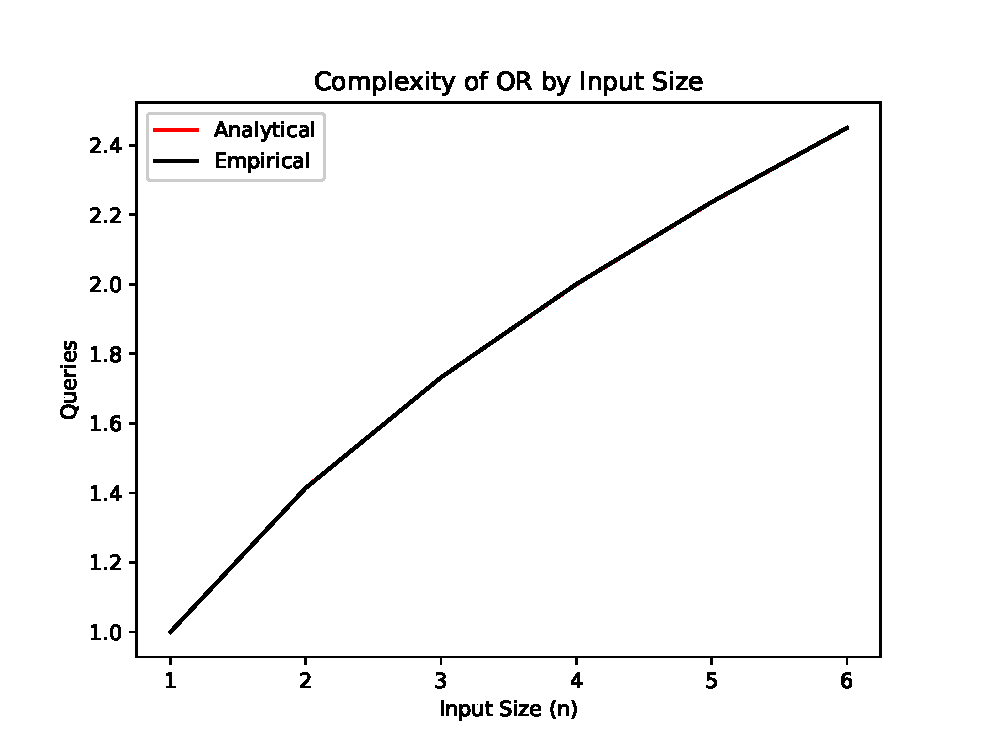
\includegraphics[scale=.5]{or_complexity}
\caption{The proven analytical optimal query complexity
and calculated empirical optimal query complexity by 
size of input bit string.}
\label{fig:or_complexity}
\end{figure}

We verify that our implementation works correctly
with results for OR on various input sizes.
The optimal quantum query complexity of OR
is $\sqrt{n}$ and, as demonstrated in
\cref{fig:or_complexity},
we the empirical results match the analytical
to the thousandth place.

\begin{figure}[H]
\centering
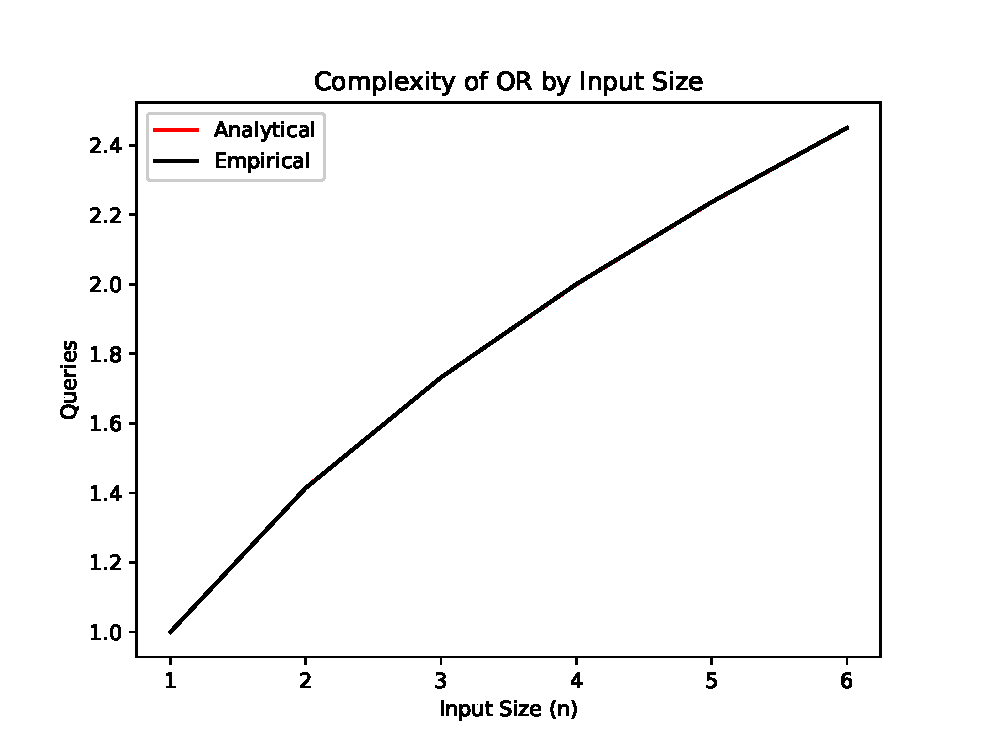
\includegraphics[scale=.5]{or_complexity}
\caption{The proven analytical optimal query complexity
and calculated empirical optimal query complexity by 
size of input bit string.}
\label{fig:or_complexity}
\end{figure}

\subsection{Runtime with OR}

\subsection{OR Function: Worst-case Boolean Inputs}\label{sec:speed}



\begin{figure}[H]
\centering
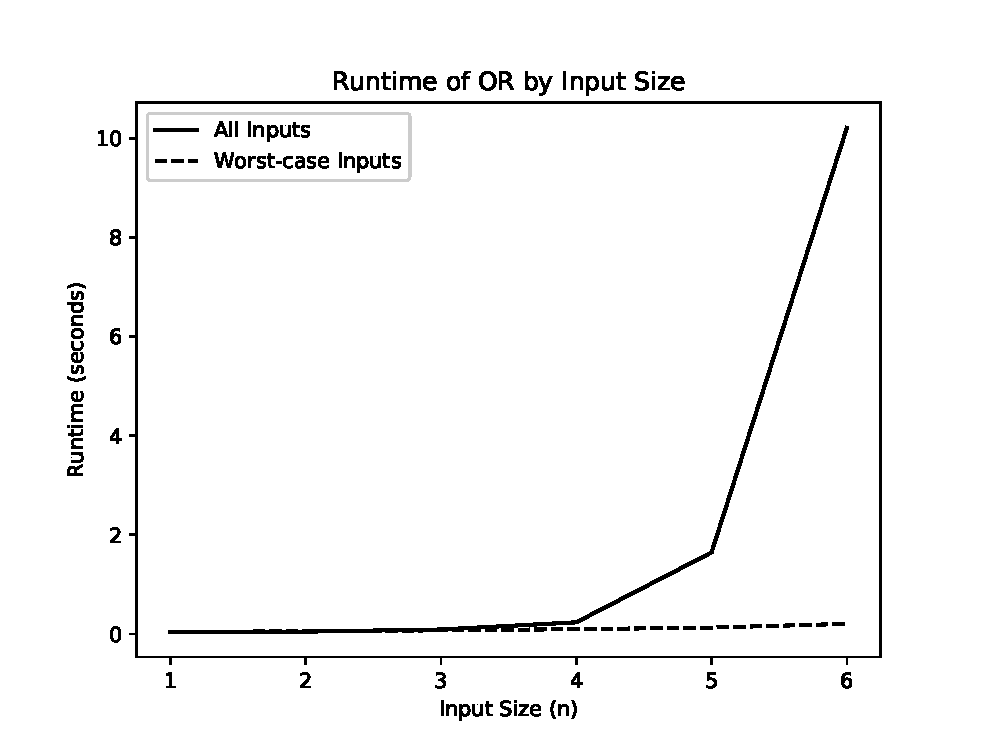
\includegraphics[scale=.5]{or_runtime}
\caption{Runtime of SDP solver by size of input strings.}
\label{fig:or_all_runtime}
\end{figure}

In \cref{fig:or_all_complexity}, observe that our algorithm
correctly calculates the optimal query complexity of the OR function (the
analytical and empirical lines are so close that one
is mostly obscured).
Our algorithm's performance is displayed in \cref{fig:or_all_runtime}.
We see that runtime grows exponentially with respect to input size as expected, 
given the exponential increase in the cardinality of the set $D$ of all
inputs of length $n$. 
We also see that our algorithm is accurately calculating the
optimal quantum query complexity of the OR function. 

The correctness of our algorithm is supported 
by it's performance on the OR function as it 
exactly matches the theoretical values. 
This is further supported by the proofs of Reichardt, 
Wen, and our Methodology section. 
In addition, we have made our source code 
available on GitHub for review. 
Given the correctness of our algorithm, 
we can address improvements to its runtime.

First, we can attempt to improve runtime while
maintaining the correctness of the algorithm. Later,
we might be able to alter the algorithm
mathematically to take advantage of the structure
given in SDP's formed from quantum algorithms. 
It has also been claimed that the dual of this semidefinite
programming problem yields the quantum algorithm with minimal query complexity.
However, this optimal solution to the dual may not be easily 
interpreted as an algorithm as there could be many optimal, feasible solutions. 
Semidefinite programming problems also don't guarantee the tightness of the dual,
as is the case in linear programming. 
These problems all pose potential areas of future expansion.

\subsection{OR Function: All Boolean Inputs}

A simple approach to speeding up the runtime of our
algorithm is to simply decrease the number of input
strings considered for a given input size $n$. It's
important that we still obtain a good approximation
of the correct answer, so we need to ensure that the
inputs we do analyze will lead to the correct result.
Because the bounds of our algorithm are adversarial,
meaning that they are worst-case bounds, we can opt
to only use the worst-case inputs.

Again returning to our OR example, the hardest inputs are
either entirely zeros, or contain only a single 1. 
Using these inputs, we can then run our algorithm to 
compare both runtime and precision of results.

The runtime is drastically improved over the all-case scenario. 
This result is not only shown via \todo{put both runtimes on the same figure and reference it here} of the graphs, 
but also in the x-axis because the speed up was so 
significant that we were able to solve for many more 
input sizes than in the all-case scenario. 
Looking at the optimal query complexities returned, 
we observe that we are still obtaining good 
approximations of the true value. 
We believe that more iterations could drastically 
improve the performance of the algorithm as well as 
improved stopping conditions. Instead of simply stopping 
after some number of iterations (in this case 100), 
we could look to see if the improvements to the objective 
function are negligible and conclude that the algorithm has converged.

\section{Conclusion}


\begin{acks}
The authors would like to thank Professors Shelby Kimmel
and Philip Caplan for their invaluable help and support. 
\end{acks}

% select the reference format (leave this)
\bibliographystyle{ACM-Reference-Format}

% specify the bibliography (.bib) file
% place your references in this bib file
\bibliography{main}

\end{document}